\chapter{Design}\label{chap:design}

% This chapter takes inspiration from existing deployment patterns for microservices discussed in the previous chapter(BACKGROUND), which leads onto the creation of an architecture, comprising of multiple modules which are used to deploy, test and analyse different deployment patterns using a series of applications.  

% To create the final architecture, the application's deployment and testing have been split into two components allowing them be modular which increase's ease of use, which is then followed by the analysis component where collected data is converted to human readable information. 
% =======

% This chapter discusses the architecture required to create a suitable testing environment to deploy, test and analyse patterns on a cloud platform. 

% To create the final design for the architecture, it has been split into multiple components, where the components deploy, test and analyse the different patterns. 

% =========
This chapter discusses the design of the architecture required to create a suitable testing platform which builds up from the requirements discussed in the chapter \ref{chp:AnR}. The architecture is split into three different components, allowing it to deploy, test and analyse different patterns on a cloud platform. 

(Probs add a section above this which discusses why you need to deploy a pattern and that it requires different applications?)
\section{Components}
% % % % % % % % % % % % % % % % % % % % % % % % % % % % % % % % 

\begin{figure}[H]

\begin{minipage}{.5\linewidth}
\centering
\subfloat[Application Component]{\label{fig:application_comp}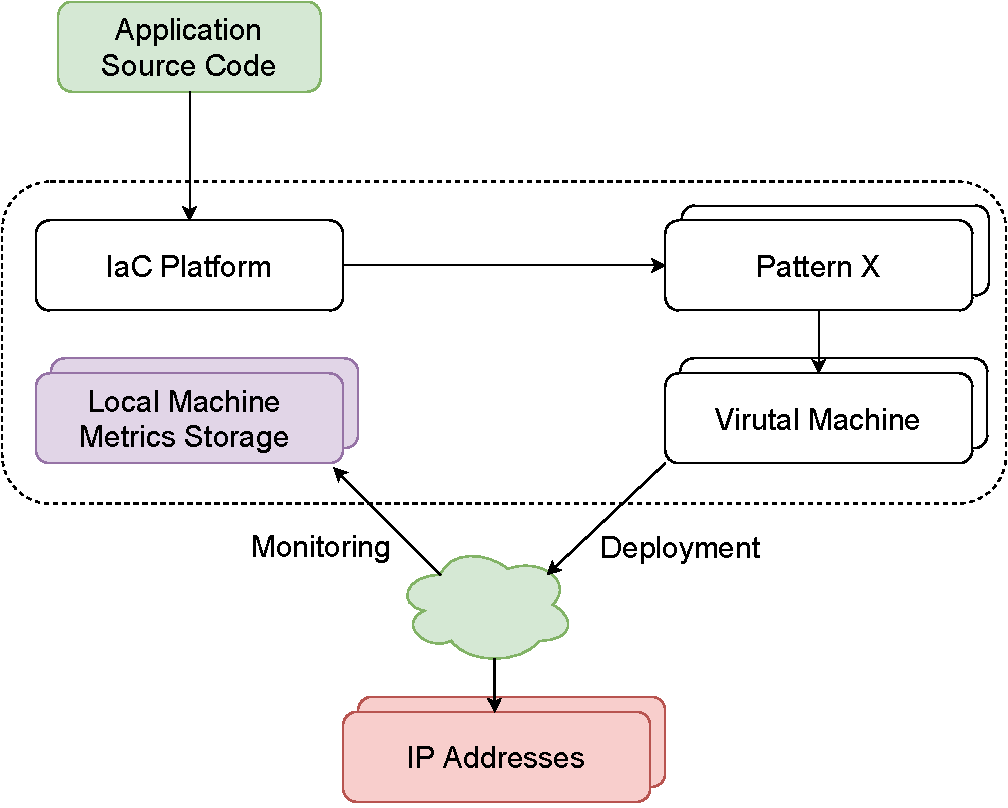
\includegraphics[scale=.36]{images/Modular_Application.pdf}}
\end{minipage}%
\begin{minipage}{.5\linewidth}
\centering
\subfloat[Testing Component]{\label{fig:testing_comp}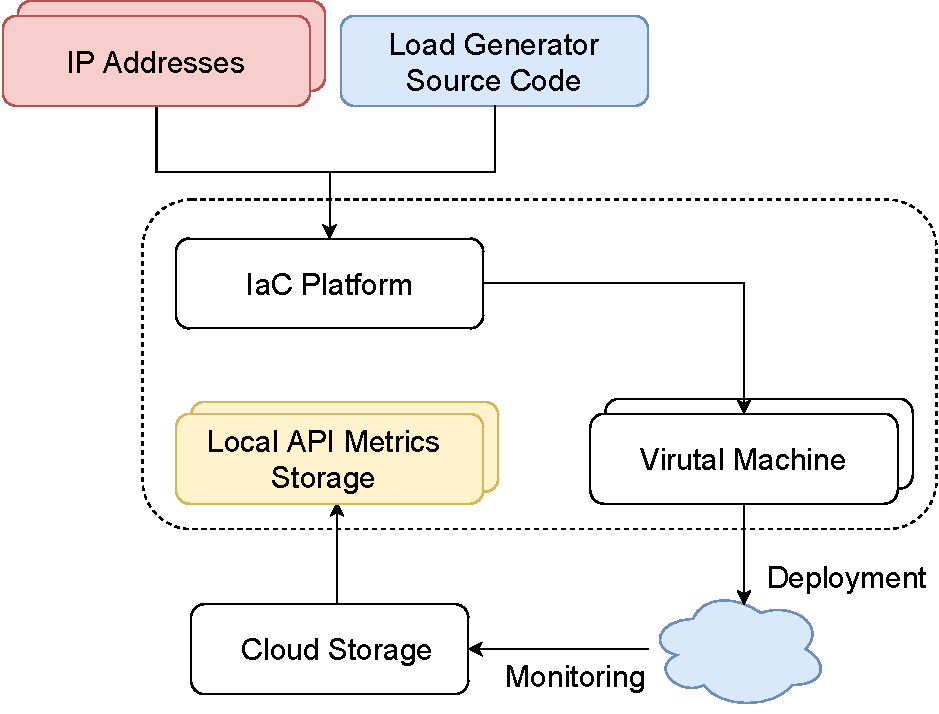
\includegraphics[scale=.4]{images/modular_load.pdf}}
\end{minipage}\par\medskip
\centering
\subfloat[Data Analysis Component]{\label{fig:analysis_comp}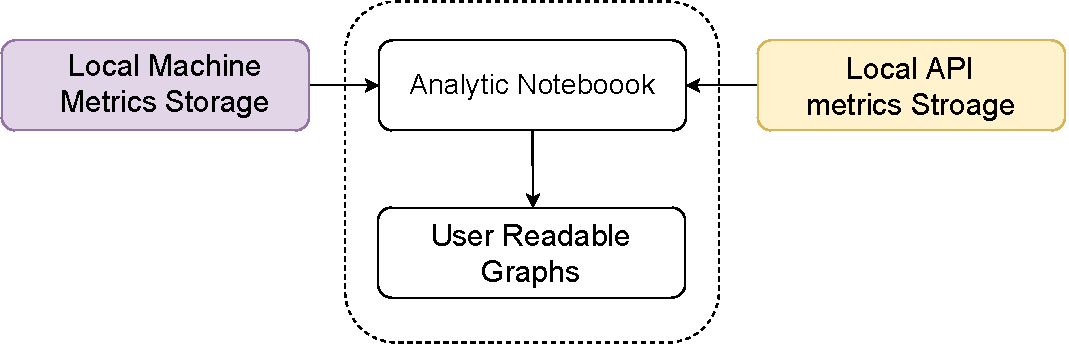
\includegraphics[scale=.4]{images/Data Flow.pdf}}
\caption{Three separate components which are used in the final architecture.}
\label{fig:main}
\end{figure}

% % % % % % % % % % % % % % % % % % % % % % % % % % % % % % % % 
\subsection{Application Component}
% \begin{figure}[H]
%     \centering
%     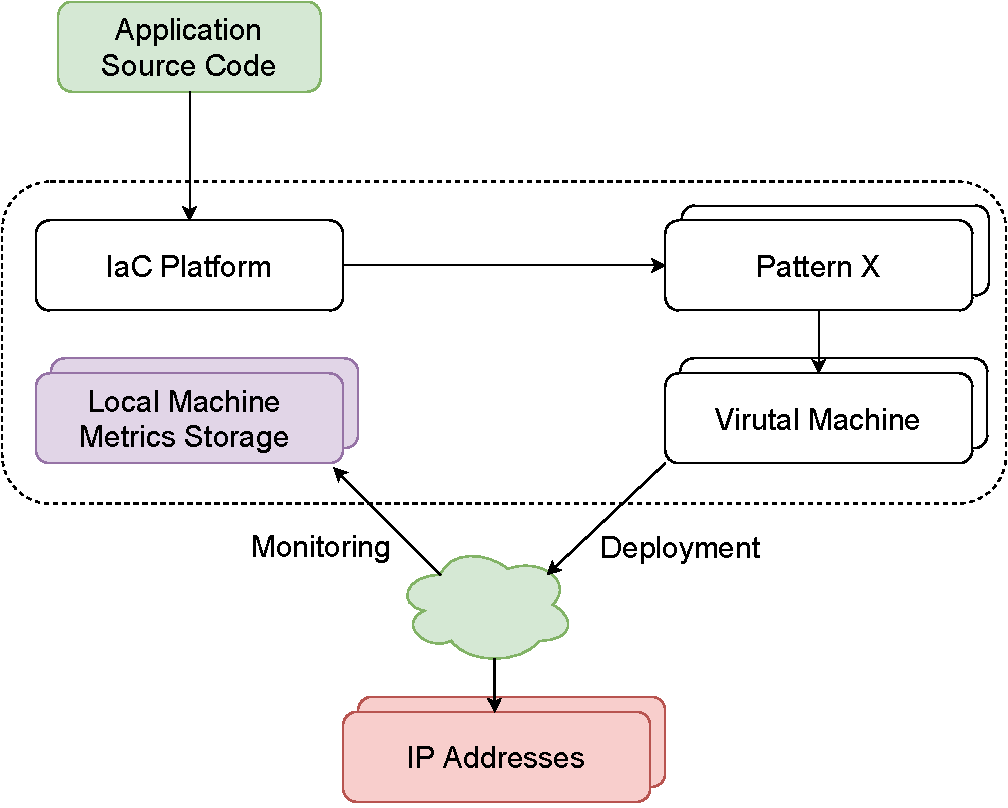
\includegraphics[width=0.7\linewidth]{images/Modular_Application.pdf}
%     \caption{Application component example using Pattern 1.}
%     \label{fig:application_comp}
% \end{figure} 

The component, as shown in sub-figure \ref{fig:application_comp}, accepts application source code, which is provisioned by the IaC platform to create multiple virtual machines within the chosen pattern to the cloud. Followed by an output of new host IP addresses, to be used by the testing component. 

A modular design of such allows for the IaC platform to create multiple machines at a time, which can be used for executing multiple tests, helping in reducing time. Once the applications have been deployed to the cloud, the module is set to an ideal state.

Followed by the creation of the testing component and after that component has been completed, this component collects the machine metrics from the cloud provider storing them locally, followed up by clearing up all instances of the component in the cloud. 
% % % % % % % % % % % % % % % % % % % % % % % % % % % % % % % % 
\subsection{Testing Component}
% \begin{figure}[H]
%     \centering
%     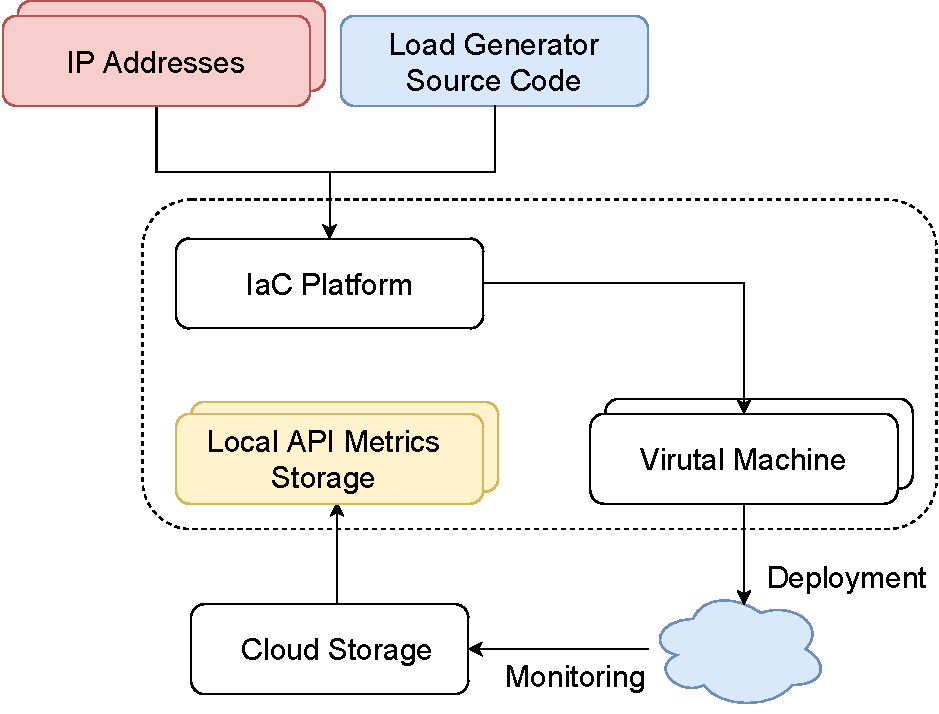
\includegraphics[width=0.7\linewidth]{images/modular_load.pdf}
%     \caption{Load Generator Component}
%     \label{fig:testing_comp}
% \end{figure} 
The component, as shown in figure \ref{fig:testing_comp}, the component accepts a list of host IP addresses generated by the application component, and the load generators source code. The list of IP addresses are now used by the IaC platform to create subsequent virtual machines which install the load generator and are then used to generate load for the deployed applications.

Once the load generator's have finished generating load, the output log file(s) are uploaded to the cloud storage, which are later downloaded locally. This is followed by clearing up all instances of the component in the cloud. 

% % % % % % % % % % % % % % % % % % % % % % % % % % % % % % % % 
\subsection{Analysis Component}

The analysis component shown in figure \ref{fig:analysis_comp}, reads in the machine's system metrics, such as memory usage and CPU usage, generated by the application component and load testings log files generated by the testing component, to create meaningful user readable information, this can be represented in a multitude of ways such as graphs or tables. 

\section{Final Architecture}
\begin{figure}[H]
    \centering
    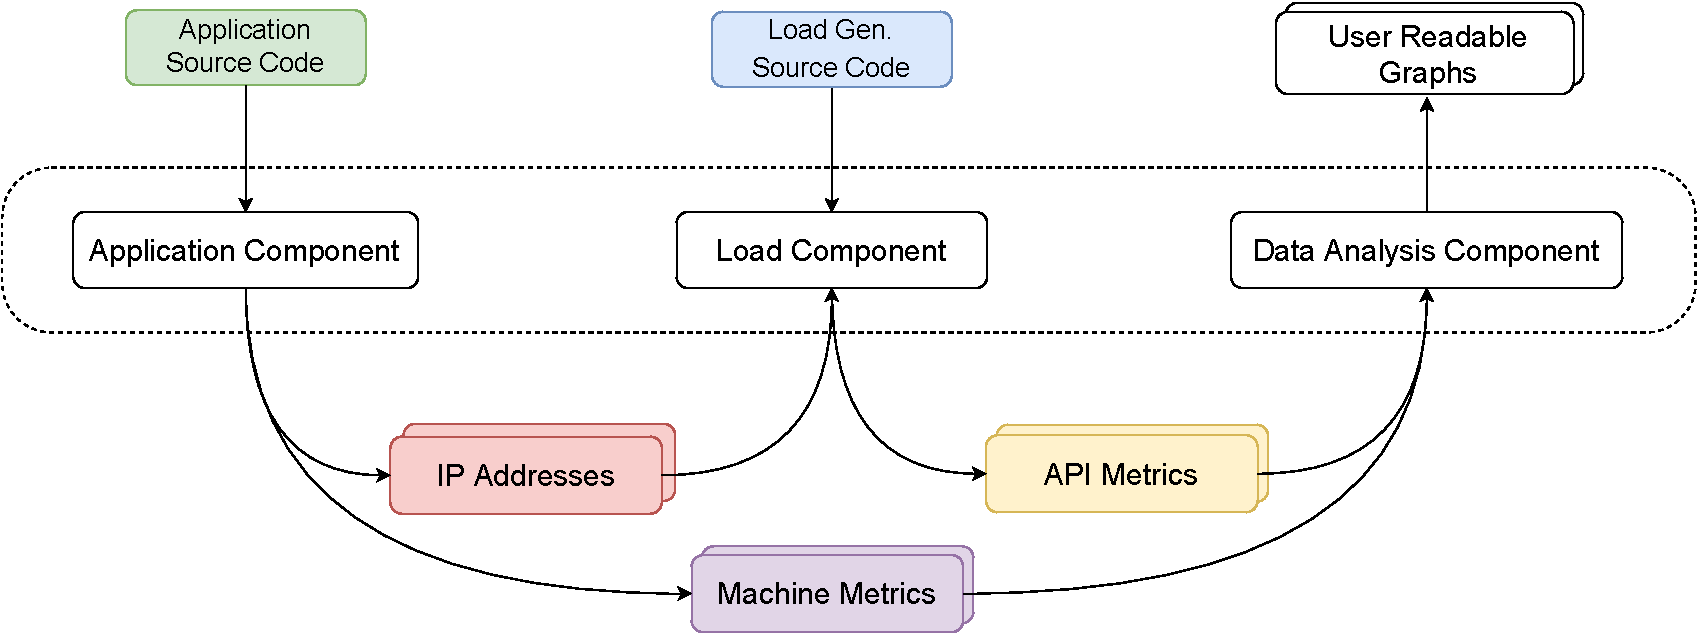
\includegraphics[width=1\linewidth]{images/final_arch.pdf}
    \caption{The final architecture, showing flow of information between each component.}
    \label{fig:final_arch}
\end{figure} 
The different components creates the final architecture as shown in figure 4.2, which outlays the various interactions between the components, the flow starts from the left side, ending to the right. (Should probs talk about how the integrations work, but unsure if that is needed) 

% The flow starts with a packaged microservice application, possibly stored on a version control system, where the source code for the application and load generator is kept separate from each other whilst also being easily accessible. 
% \\
% The source code follows two paths, controlled by the Main Script, where 
% \\
% \hspace*{6mm} \textbf{Path A} flows into the Infrastructure as a Code (IaC) platform which boots up a suitable virtual machine based on the requirements, such as deploying Pattern's one or two, which require modifications in the IaC script, once a machine is booted, the application can be hosted within the machine returning the Host's IP address with the application forwarded to the port address.
% \\
% \hspace*{6mm} \textbf{Path B} follows a similar path, however, skips out on the patterns, and is created after the application machine is hosted. Path A and B collide at this point, where B takes in the Host IP Address, and runs the load generator scripts for a certain amount of time, saving this data to the cloud provider so it can later be downloaded locally. 

% This is where the unit A's machine metrics are pulled from the provider and stored locally side by side to the API metrics. This concludes the use of both cloud machines and can be safely dropped. At the last stage of the workflow, both paths with the machine and API metrics flow into the analytical notebooks where data can be made sense of and compared to. 

